\documentclass[12pt]{report}
\linespread{1.5}
\usepackage{graphicx}
\usepackage{fullpage}
\usepackage{natbib}
\usepackage{float}
\usepackage{subfig}

\bibpunct{[}{]}{,}{a}{,}{,}

\begin{document}

\title{Developing a Compiler for the Expert Systems Language, Flex}
\author{05017742 - Thomas Cowell\\
		\texttt{05017742@glam.ac.uk}}

\maketitle

\begin{abstract}
The aim of this project is to create a simple compiler for the expert systems language, Flex.  Flex is an expert systems language that focuses on using plain English to make it accessible for non-technical users, and to aid building rapid rule based systems.
\end{abstract}

\pagestyle{plain}
\pagenumbering{alph}

\tableofcontents

\cleardoublepage
\pagenumbering{arabic}

\chapter{Introduction}

\section[Why This Project?]{Why This Project?}\label{sec:why_this_project}
Before this paper begins, it is worth noting the motivation behind this project.  Certain modules on the 'Intelligent Computer Systems' course required the use of a propietary software package called WinProlog.  The application can do a wealth of tasks, however, the modules only focused on a niche feature of the software, a toolkit based on Prolog called Flex (not to be confused with the lexical analysis tool, or Adobe's Software Development Kit, also of the same name).  Win-Prolog's Flex allows professionals, engineers and students alike to quickly write a rule-based system using a language that is very close to the English language.
\\*
\\*
Whilst flex achieved results, it was felt that the debugging features were sub-par and were often inaccurate, giving no helpful messages for a beginner to use to correct their mistakes.  Also, because of the restrictions of having a licence, it meant that the software could only be installed on certain machines, in a different department within the University campus, which students felt was restrictive and inconvienient.
\\
\\
\\
\\
\begin{figure}[h!]
	\centering because empathy doesn't support otr. pidgin for icq xmpp(jabber). smuxi f
		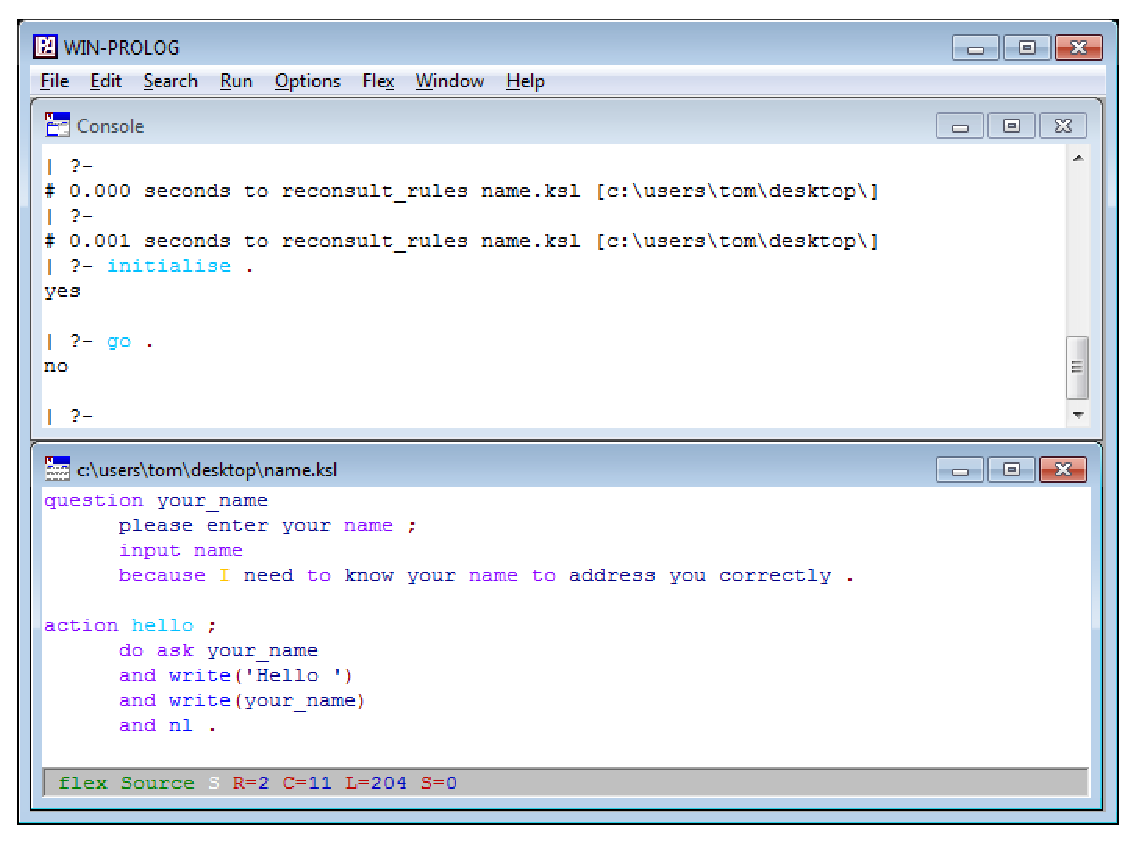
\includegraphics[scale=0.85]{flexfail}
		\caption{A simple flex program that is syntatically wrong, plus the resulting error.}
\end{figure}
\\
In figure 1.1, the line \texttt{input name} should have a semi-colon at the end, like \texttt{input name ;}, to let the compiler know that the line is finsihed, but the question isn't over.  Whilst this is a simple mistake, the flex compiler hasn't picked it up, and is only being discovered when trying to run the action \texttt{go}, where flex returns an error message \texttt{no}, with no indiciation what the error is, where it is or how to fix it.  If this were a large set of rules, finding such a basic mistake could take a long time to fix.
\\*
\\*
The examples below show flex encountering a gramatically incorrect script, with the compiler displaying errors.
\begin{figure}[h]
	\centering
		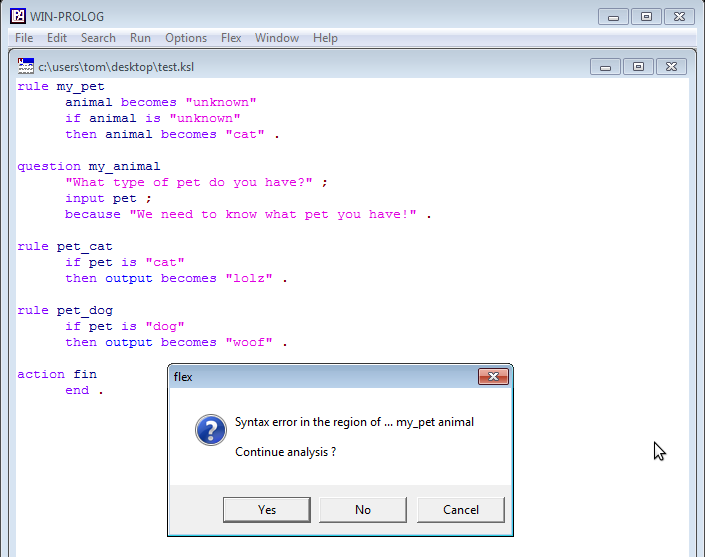
\includegraphics[scale=0.65]{flex_error1}
		\caption{The compiler has detected an error in the grammar.}
\end{figure}
%\\*
%\\*
What we see here is some random text talking about nothing much at all!
\begin{figure}[ht]
	\centering
		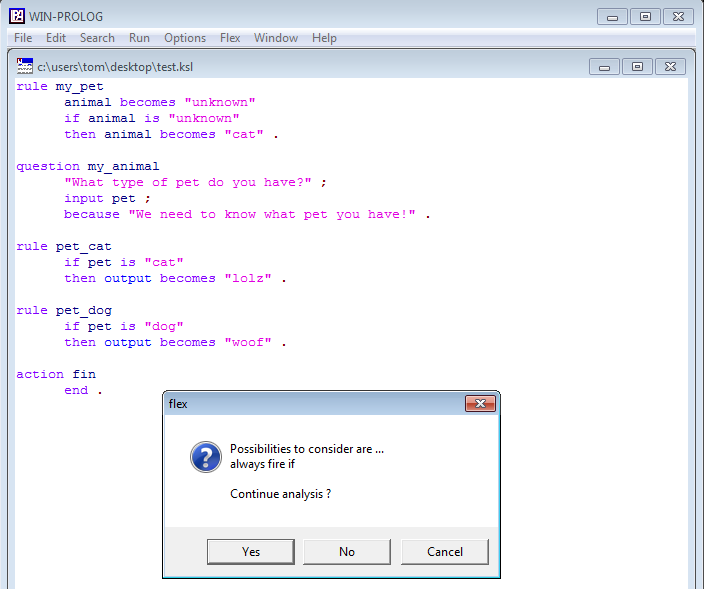
\includegraphics[scale=0.65]{flex_error2}
		\caption{The compiler error isn't very specific to where it is refering to, there are no line number or highlighting on the error.}
\end{figure}
\\*
Whilst the compiler in WinProlog does try to track down the error, it's not very friendly to new users, as it doesn't let them know where the error is, or what is wrong.  There were situations where n tutorials and in courseworks, where by small, simple errors could have been easily fixed if it weren't for ambiguous language on the debugger.
\clearpage
\section{Aim}\label{sec:aim}
The problems outlined in the previous section help highlight the aims and objectives that this project can use.  Time is limited, so it wouldn't be wise to implement a full version of Flex, however a small subset of the language would be sufficient.
\\
\\
This project aims to create a basic implementation of the flex toolkit, using open source software.  The software would be able to be installed on any linux machine, whilst providing the basic features required to teach students how to write expert systems.
\section{Objectives}\label{sec:objectives}
The objectives of this project are to:
\begin{itemize}
\item Create a simple flex interpreter that can work on the simple tutorials from a tutorial.
	\begin{itemize}
	\item Recognise rules, questions and actions;
	\item Recognise variables, assignments and comparisons;
	\item Work with simple if-statements
	\item Output variables and text using the write() statement.
	\end{itemize}
\item Create it for the Linux platform.
	\begin{itemize}
	\item Command line driven - feed the application a flex source file.
	\item Not be coupled to a Desktop Environment (Gnome, KDE etc).
	\end{itemize}
\item Keep the project open source.
	\begin{itemize}
	\item Keep the project available on a source-control service so it can be ammended to once the project is finished.
	\end{itemize}
\end{itemize}

\section{Project Overview}\label{sec:project_overview}
This project shall begin by looking into the previous or similar research that others have carried out on this topic.  Reseach will then be conduced into Expert Systems, Win-Prolog and flex, with sample scripts of what it is capable of.  Adding to this, research will then be conducted into the tools used to write a compiler.  The implementation of the compiler will also be documented.

\chapter{Literature Review}
\section{Outline}\label{sec:outline}
As described in the previous chapter, the outline of this project is to create a compiler for the expert systems language, flex.  Whilst Flex is based on the Artificial Intelligence langauge Prolog, this basic compiler will be written in C, emulating the basic features of flex, mainly as a teaching tool, rather than a fully fledged toolkit.  However, because Flex is built on top of Prolog, there are many papers on writing Prolog compilers.

\section{Previous Work}\label{sec:previous_work}
Because the Flex toolkit is unique, there aren't many examples or previous work done on creating a compiler soley for Flex.  However, there are countless items of literature dedicated to writing compilers, all for different languages, but constructed in the same manor - using Flex and Bison.

\chapter{Research}
\section[Research]{Research}\label{sec:intro_to_research}
Before any implementation can begin, research needs to be conducted in order to gain better knowledge about expert systems, the Flex language and various toolkits for developing interpreters.

\section{Artificial Intelligence}\label{sec:AI}
Artificial Intelligence (AI) is a term for machines that can appear to act as if they are 'thinking' for themselves - that is, to emulate the way the human mind works.\\
\\
Roughly speaking, Artificial Intelligence is the study of man-made computational devices and systems which can be made to act in a manner which we would be inclined to call intelligent. \citep{whatisai}
\\
\\
Interest in AI began when the British computer scientist Alan Turing stated, that if a machine can pass a series of questions, and trick the questioner into thinking that the machine was infact human, then the machine could be classed as having intelligence.  This test has since become known as the 'Turing Test'.\\
\\
Expert Systems fall into the category of AI, because they emulate the roll of an expert of a field.  Given answers, an expert system should be able to come to a conclusion based in varying pieces of information.
\section{Expert Systems}\label{sec:expert_systems}
In the modern world where information is highly valuable and where time is of the esence, many experts have turned to computing to help provide answers for them that may otherwise take a while to reach through their own expertese.  Expert Systems provide an easier way for professionals to reach conclusions through a series of questions, usually linking to a knowledge base.  For example, a doctor may use an expert system to reach a diagnosis for a patient, where the illness or problem may not be readily obvious.  The system would ask a question, where the doctor would answer with the symptoms, and then the expert system would continue asking more questions, based on the previous answers, until a conclusion is reached.
\\*
\\*
Expert system development entials the conversion of information about a bounded problem domain into knowledge, which is then represented in a format suitable for computer manipulation.  The created depository of knowledge, known as the knowledge base, can then by used by various deductive reasoning techniques to derive solutions \citep{expertsystems98}.
\\*
\\*
From this, it is obvious that the usefulness of the expert system is only as good as the underlying data - the knowledge base.  Using the doctors example from the previous paragraph, the system would be of no use if the knowledge base was minimal, whilst in the reverse situation, it would be extremely useful to have a large knowledge base.  Doctors from around the world could contribute answers as new illnesses and cures are discovered, which in turn would improve the accuracy and usefulness of the expert system.
\\*
\\*
Expert systems can be found in many areas of industry, including engineering, medical, financial forecasting, or even just personal information systems for helping customers at a shopping centre.
\\*
\\*
Expert systems languages are entirely different to imperative languages such as C, C\#, Java.  Instead, they make use of logical langauges, such as Prolog, which is based on rules, and assosciations with data.  The code in figure \ref{fig:prolog_code} shows a short example of a program written in Prolog.
\\*
\\*
\begin{figure}[H]
\texttt{born(charles, elizabeth2, philip).\\
born(anne,    elizabeth2, philip).\\
born(andrew,  elizabeth2, philip).\\
born(edward,  elizabeth2, philip).\\
\\
born(diana,   frances,    edwardSpencer).\\
\\
born(william, diana,      charles).\\
born(henry,   diana,      charles).\\
\\
? born(S, elizabeth2, Y) and born(G, M, S).}
\caption{Example Prolog code.\citep{thehouseofwindsor}}
\label{fig:prolog_code}
\end{figure}
The first four lines link the first argument with the next two.  So, on line one, charles is the child of elizabeth2 and philip.  On the 5th line, diana is declared as the daughter of frances and edwardSpencer 
The final line execute the program, by submitting a query.
\\*
\\*
\begin{figure}[H]
\texttt{born(charles, elizabeth2, philip), born(william, diana, charles) yes\\
born(charles, elizabeth2, philip), born(henry, diana, charles) yes}
\caption{Output from executing the sample code.}
\label{fig:prolog_output}
\end{figure}
Figure \ref{fig:prolog_output} shows the output from the sample code.  The query executes two sub queries, \texttt{born(S, elizabeth2, Y)}, which retrives a set of data where the child's mother is \texttt{elizabeth2}.  Based on the four rules at the start of the program, this would return four answers for \texttt{S}, and a single result for \texttt{Y} (philip).  The second query, \texttt{born(G, M, S)} queries the returned data set from the first query.  In this case, the mother (\texttt{M}), while the father is \texttt{S}.  Lines six and severn in \ref{fig:prolog_code} show that charles has two children, and thus \texttt{william} and \texttt{henry} are returned.
\clearpage
\textbf{Disadvantages}\\
There are some notable disadvantages to expert systems.  An important pitfall to consider is the GIGO acronym - Garbage In Garbage Out.  If the rules are .  Also, if the person being questioned gives an answer that they're uncertain of, then the result may not be accurate, and the expert system would be non-the wiser.  A human expert would be able to tell the certainty of someones answer, and possibly re-ask the question in a way that the questionee would understand.

\subsection{WinProlog}\label{subsec:winprolog}
WinProlog is a propietary software package, developed by Logic Programming Associates Ltd.  LPA describe Win-Prolog below:
\\*
\\*
WIN-PROLOG is the leading Prolog compiler system for Windows-based PCs. Prolog is an established and powerful AI language which provides a high-level and productive environment based on logical inference.\citep{lpawinprolog}
\\*
\\*
One of the features of Win-Prolog is Flex, an expert systems toolkit built on top of Prolog.

\subsection{Flex}\label{subsec:introflex}
The 'Flex Tutorial' describes Flex as "Flex is a software system specifically designed to aid the development and delivery of Expert Systems."
\\*
\\*
To appreciate both the power and limitations of Expert System approaches to reaching expert conclusions, it is necessary to construct and experiment with expert systems.  In this module, the Flex Expert System Shell will be used.  Flex describes knowledge in terms of \textit{production rules} (that is, \textit{if-then} statements), which has proved the most popular approach to encapsulation expert knowledge.  Such rules, despite appearing simple, enable relatively complex connections to be made between individual pieces of 'knowledge', thereby solving apparently difficult problems.\citep{flexsystems09}.
\\*
\\*
The advantages of flex is that it's easy to understand, as it's very close to the English language.  A non-programmer could look at it and understand the system within several minutes, where as a traditional Prolog script may need some understanding of programming to be able to understand what is going on.
\\*
\\*
Flex expert system toolkit, an expressive and flexible rule-based development system for building and delivering scalable and flexible expert systems and business rules applications. Flex provides a comprehensive and versatile set of facilities for both programmers and non-programmers to construct reliable and maintainable applications.\citep{lpawinprolog-flex}.
\\*
\\*
The code below shows an example program written in flex:
\begin{figure}[H]
\texttt{\begin{tabbing}group \= temperature\_choices warm, cold .\\
\\
rule ask\_temperature \\
\>	if the temperature is unknown\\
\>	then ask temperature .\\
\\
question temperature\\
\>	What is the temperature?;\\
\>	choose from the temperature\_choices ;\\
\> 	because it is necessary to work out the need for a coat .\\
\\
rule temp\_w\\
\>	if temperature is warm\\
\>	then write('You would be mad to wear a coat.').\\
\\
rule temp\_c\\
\>	if temperature is cold\\
\>	then write('Take a coat to keep warm.').\\
\\
ruleset take\_a\_coat\\
\>	contains all rules;\\
\>	select rule suing first come first servced;\\
\>	update ruleset by removing each selected rule;\\
\>	initiate by doing restart .\\
\\
action go\\
\>	do invoke ruleset take\_a\_coat .\\
\end{tabbing}}
\caption{A simple flex program that lets you know if you should wear a coat or not.\citep{flexsystems09}}
\label{fig:flex_code}
\end{figure}
It's immediately obvious that the program is made up of rules and questions.  The compiler starts from the top, and runs down through the rules, until they've all been fired.  Questions only get fired if they are called upon within a rule.\\*
\\
The first line declares a group of choices that can be asked during a question.  This can be likened to a Enumerative type in languages such as C and C\#, where \texttt{warm} and \texttt{cold} are two options that belong to \texttt{temperature}.  The first rule, \texttt{ask\_temperature}, checks if the variable \texttt{temperature} (not to be confused with the group of the same name) has been assigned a value.  If it's not, then it asks the question, \texttt{temperature}.  Because the flex compiler starts at the top, then temperature will be unknown by default, so this rule will always fire.\\
\\
Questions always have the same format: The first line is the question text that the user will see, the second line presents the options to the user and also accepts their input.  In this instance, the user will be presented the two choices of \texttt{temperature}, where the choice is then assigned to the variable \texttt{temperature}.\\
\\
The two rules, \texttt{temp\_w} and \texttt{temp\_c}, check the users input, and display the message as appropriate, while the ruleset \texttt{take\_a\_coat} tells the compiler how to go about running the script.  Finally, the the action \texttt{go}, which is triggered as a query from the command prompt, starts the program.\\
\\
Whilst this is a reasonably simple script, it has all the basics that make up larger and more complicated flex programs.

\section{What Is A Compiler?}\label{sec:what_is_a_compiler}
Programming languages are notations for describing computations to people and to machines.  The world as we know it depends on programming langauges, because all the software running on all the computers was written in some programming langauge.  But, before a program can be run, it first must be translated into a form in which it can be executed by a computer.

The software systems that do this translation are called \textit{compilers}.\citep{compilers07}
\\*
\\*
This quote nicely gives a brief overview of what a compiler does.  It translates the human readable program into a format that the computer can understand, i.e. instructions.  Whilst this sounds simple, the actual process is reasonably complicated, and done in several phases:\\
\begin{itemize}
	\item Lexical Analysis
	\item Syntactical Analysis
	\item Intermediate Code Generation
	\item Optimization
	\item Object Code Generation
\end{itemize}\citep{compilerconstruction92}
\subsection{Lexical Analysis}\label{subsec:lexical_analysis}
The first task of the compiler is to read the source code that the developer has written, and breaks it up into meaningful chunks called tokens.  These tokens are defined in a lexical file, in which the lexical scanner will process.
\\*
For example, take the following flex code:\\*
\texttt{\begin{tabbing}rule \= my\_pet\\
\>	if animal is 'cat'\\
\>	then sound becomes 'meow' .\\
\end{tabbing}}
This can be broken down to be easier to understand:\\*
\begin{itemize}
	\item keywords: rule, if, is, then
	\item identifiers: my\_pet, animal, sound
	\item operator: becomes
	\item string: 'cat', 'meow'
	\item punctuation: .
\end{itemize}
The lexical analyiser is capable of removing characters that aren't relevant to the program, such as comments, new lines and whitespace (spaces and tabs).  All of the above are leximes that are mapped into tokens, that makes it easier for the syntactical analyser to understand.  The way that the lexical analyser recognises these leximes is through matching the patterns of text, which is where regular expressions come in useful.\\
\subsubsection{Regular Expressions}\label{subsubsec:regex}
Regular Expressions, or more commonly known as 'regex', allows developers to match patterns of text.  It is extremely powerful for recognising patterns in text, and thus, is used in the lexical analysus process for matching expressions to create tokens.
\\*
\\*
A regular expression is a pattern description using a metalanguage, a language that you can use to describe what you want the pattern to match.  Flex's regular expression language is essentially POSIX-extended regular expressions (which is not surprising considering their shared Unix heritage).\citep{flexandbison09}
\\*
\\*
Regular expressions are a powerful way of matching complicated patterns of strings.  It uses a series of special characters that allow the user [of regular expressions] to create a query.
\\*
For example, numbers can be expressed in several ways, some numbers are negative and some have decimal places.  An expression needs to be able to recognise these different formats.  A string of digits, which can either be positive or negative, can be represented using the expression below:\\*
\\*
\texttt{[-+]?[0-9]+}
\\*
\\*
The square brackets \texttt{[ ]} represents a character class, matching anything within the brakcets.  The first occurance, \texttt{[-+]} matches either a postive of a negative symbol at the start of the expression.  The \texttt{?} character means that the preceding character class can either occur once, or never, which means that the plus or minus characters can be optional.  Next is the \texttt{[0-9]} expression, which matches any text that is number 0 to 9 - the \texttt{+} at the end means that the preceeding expression can be matched one or more times, allowing a number to be either 1 or 12345.  Another example, shown below, recognises an identifier, such as one from the flex example.
\\*
\\*
\texttt{[a-zA-Z\_][a-zA-Z0-9\_]*}
\\*
\\*
The expression is comprised of two character classes.  The first matches a series of characters, in either lower or uppercase, followed by an underscore. The following class is similar, but can also contain numbers.  The astricks, \texttt{*}, means that the preceeding expression can be matched zero or more times, so, the second character class is optional.  This example allows for an identifier to look something like:\\
\\
\texttt{animal}\\
\texttt{My\_Animal01}\\
\texttt{animal\_}\\
\\
But \textbf{not}:\\
\texttt{my1\_animal}\\
\texttt{1\_animal}\\
\\
Matching keywords is much easier, as they need to be treated literally.  Matching for the \texttt{if} keyword, for example, simply looks like so:\\*\\*
\texttt{"if"}
\subsection{Syntactic Analysis}\label{subsec:syntactical_analysis}
The process of syntactic analysis is to parse the tokens into meaningful sentences.  It creates a tree of tokens, whereby each node represents an operation such as \texttt{while}, and its child nodes represent the evaluation expression, and the block of code to loop around, which could be broken down again, where the evaluation is the root node, and the children are the parameters and comparison operators.
\begin{center}
\texttt{\begin{tabbing}while \= (found != true) \{\\ \> found = do\_something();\\ \}\end{tabbing}}
\end{center}
The code above can be broken down into tokens.
\begin{itemize}
	\item Keywords: while, true
	\item Identifiers: found, do\_something
	\item Operators: =
	\item Comparison: !=
	\item Punctuation: \{ \} ( ) ;
\end{itemize}
\begin{figure}[H]
	\centering
	\includegraphics[scale=1]{whilegraph}
	\caption {Expression parse tree.}\label{fig:whilegraph}
\end{figure}
Figure \ref{fig:whilegraph} shows a parse tree of the simple \texttt{while} code sample.  The code is broken down into two main parts - the evaluation, and the block.  These are then further broken down further down the tree.
\\*
The syntactic analyzer, or \textit{parser}, is the heart of the front end of the compiler.  The parser's main task is analyzing the structure of the program and its component statements and checking these for errors.  It frequently controls the lexical analyzer, which provides tokens in response to the parser's requests, and it may also supervise the operation of the intermediate code generator.\citep{compilerconstruction92}
\\*
\\*
A programming langauge follows a strict set of rules that form it, much like the English langauge has rules to string certain words together to form meaningful and sensible sentences.  The parser's job is to put the tokens into an order that follows the grammar.  For example, the grammar specifies that an identifier, or an expression, must come after the \texttt{if} keyword, followed by a comparison of another identifier or expression.
\subsubsection{Grammar}\label{subsubsec:grammar}
For the parser to operate, there needs to be a way for the syntactic analyser to convert the tokens into the parser tree.  The grammar fulfills this role by using a BNF, or EBNF.  It originally started as BNF (Backus-Naur Form), as created by John Backus and Peter Naur to describe the syntax of a specific language.\\*
\\*
John Backus and Peter Naur introduced for the first time a formal notation to describe the syntax of a given langauge (This was for the description of the ALGOL 60 programming langauge. \citep{whatisbnfnotation}
\\*
\\*
The grammar is the important area of the parser, as it defines how the langauge should look and work.  Most langauges use "context free grammars", where the grammar is built up of small chunks, which can be used in themselves.\\*
\\*
Context-free grammars are used to describe the syntactic structure of programs of a programming language.  This shows how programs are composed from subprograms, or, more precisely, which elementary constructs there are and how composite constructs can be built from other constructs. \citep{compilerdesign95}\\*
\\*
Take the following EBNF grammar for example:\\*
\begin{figure}[H]
\begin{tabbing}
\texttt{stmt:}\= \texttt{ if\_stmt}\\
\>\textbar \texttt { while\_stmt}\\
\>\texttt{;}\\
\\
\texttt{if\_stmt:}\= \texttt{ if test then expr else expr}\\
\>\textbar \texttt{ if test then expr}\\
\>\texttt{;}\\
\\
\texttt{while\_stmt:}\= \texttt{ while '(' test ')' '\{' expr '\}'}\\
\>\texttt{;}\\
\end{tabbing}
\caption{Conext Free Grammar in EBNF}\label{fig:context_free}
\end{figure}
Figure \ref{fig:context_free} shows three rules, \texttt{stmt}, \texttt{if\_stmt} and \texttt{while\_stmt}.  The root rule here, \texttt{stmt}, contains two further rules, which can either be an if statement, or a while statement.  These statements are then declared seperately below, where \texttt{if\_stmt} declares two types of if statements that is allowed.  The if statement can either consist of an if-then-else, or an if-then statement.  These rules also contain other rules nested inside of them, such as \texttt{test} and \texttt{expr}, however they aren't listed for the purpose of the example.
\subsubsection{Parsing}\label{subsec:parsing}
Parsing is the process of constructing the parse tree from the grammar.  There are two different ways of performing this task, both of which are described below.
\paragraph{Top-Down Parsing}
The top-down parser begins with the start symbol in the grammar, and with the use of the token stream, tries to predict which is the next route to take to get to the end result.\\
\\
The top-down parser must start at the root of the tree and determine, from the token stream, how to grow the parse tree that results in the observed tokens.  It must do this from nothing but knowledge of the incoming tokens and of the productions in the grammar.  Furthermore, as a practical matter, it must scan the incoming tokens from left to right. \citep{compilerconstruction92}
\\
This quote gives a basic overview of how the top-down parsing process works.
\paragraph{Bottom-Up Parsing}
A bottom-up parser attempts to perform the parsing the opposite way of top-down, in that it starts at the leaf nodes, and works its way to the root.  Bottom-up parsing is much more powerful, but more complex, than top-down parsing.
\subsection{Intermediate Code Generation}\label{subsec:intermediate_code_gen}
Bing bish bash bosh
\subsection{Optimization}\label{subsec:optimization}
Bing bish bash bosh
\subsection{Object Code Generation}\label{subsec:object_code_gen}
Bing bish bash bosh

\section{Development}\label{sec:development}
\subsection{Environment}\label{subsec:dev_environment}
One of the main aims of this project was to create an open-source alternative to the propietary package "WinProlog", which provides the Flex toolkit.  This aim was to provide the project on an open-source platform, such as Linux, which would allow lecturers to tailor the package to their needs, allowing them to fix any bugs or add more advanced features, without the fear of violating any licences.  Therefore, Linux was the platform of choice to develop on, where the distribution of choice was Ubuntu, as it has a great wealth of development applications in its repositories, such as \texttt{flex}, \texttt{bison} and \texttt{gcc}.  Ubuntu provides a package, \texttt{build-essential}, to help developers write and compile applications easily, which contains many useful tools that should please a large majority of software developers.\\*
\\*
Installing these packages in Ubuntu simply required the following command:
\\*
\\*
\texttt{\$ sudo apt-get install flex bison build-essential}
\\*
\\*
Flex and Bison shall be discussed in the next chapter.  \texttt{build-essential} is a Debian meta-package, that is, it is simply a list of packages that are essential to building applications in a Debian based distribution.  The package satifisies the needs for most developers wishing to develop applications on Linux, and includes packages such as \texttt{gcc} and \texttt{g++} - a C and C++ compiler, respectively.
\\*
\\*
Ubuntu provides a wealth of choice when it comes to development tools, however only the simple tools are required, such as a text editor such as \texttt{gedit}, or console based text editor, \texttt{nano}, whilst the terminal is perfectly acceptable for running commands to compile the tokens, grammar and C program together.  \texttt{make} comes part of the \texttt{build-essential} package, which allows a developer to write a series of commands into a makefile, and then simply run the command:\\*\\*
\texttt{\$ make}
\\*
\\*
in the directory where the makefile is located.
\subsection{Flex}\label{subsec:flex}
Flex is a lexical analyser, which takes an input, i.e. the source code, and tokenises it ready to be parsed.\\*
\\*
There are several incarnations of lexical analysis programs, but the most popular is Flex, which originally dirived from yacc and lex.  Lex was written in 1975 by Mike Lesk and Eric Schmidt (now CEO of Google Corporation)

Flex and Bison are tools for building programs that handle structured input.  They were originally tools for building compilers, but they have proven to be useful in many other areas. \citep{flexandbison09}.
\\*
\\*
Flex was chosen due to it being a popular lexical analyser.  This has the advantage of their being lots of support and documentation for it, and it's also easily available from the Ubuntu repositories.\\*
\\*
The sample code below is an extract from the book Flex \& Bison:
\begin{figure}[H]
	\begin{tabbing}
	\texttt{/* just like Unix wc */}\\
	\texttt{\%\{}\\
	\texttt{int chars = 0;}\\
	\texttt{int words = 0;}\\
	\texttt{int lines = 0;}\=\\
	\texttt{\%\}}\\
	\\
	\texttt{\%\%}
	\\
	\\
	\texttt{[a-zA-Z]+} \> \texttt{\{ words++; chars += strlen(yytext); \}}\\
	\texttt{\textbackslash n} \> \texttt{\{ chars++; lines++; \}}\\
	\texttt{.} \> \texttt{\{ chars++; \}}
	\\
	\\
	\texttt{\%\%}
	\\
	\\
	\texttt{main(int argc, char \*\*argv)\{}\\
	\> \texttt{yylex();}\\
	\> \texttt{printf("\%8d\%8d\%8d\textbackslash n", lines, words, chars);}\\
	\texttt{\}}
	\end{tabbing}
	\caption{A word count program written in flex}\label{fig:flexwc}
	\citep{flexandbison09}
\end{figure}
The small flex program in figure \ref{fig:flexwc} counts the characters, words and lines in a given file.  It works similar to the \texttt{wc} GNU program in unix based systems.  The program is separated into three sections, by the use of the \texttt{\%\%} characters.  The first section declares any variables, such as \texttt{chars}, \texttt{words}, \texttt{lines}.  

The second section is the heart of the lexical analyser, and is where the patterns are matched to create tokens.  In this example, there are three patterns to match: a whole word, a new line, and any character at all (decipted by the \texttt{.} character).  When each pattern is matched, the variable is incremented.

The third section looks like a C program, which contains a \texttt{main} function and two lines of code.  The first line, \texttt{yylex();}, call the analyser to run on a text file that has been passed as an argument.  The second line, \texttt{printf}, outputs the values of the variables, after the lexer has been run.
\\*
\\*
The example in figure \ref{fig:flexwc} doesn't generate any tokens, as it doesn't make use of a syntactic analyser (Bison), however, they can be generated like so:
\\*
\\*
\texttt{"if"\quad\quad return IF;}\\
Where IF is the token to return.  Tokens can also be created for values and numbers.  The value is stored into yylval, which is passed to the parser, along with a token, so that the parser knows the type.
\\*
\\*
\texttt{[0-9]+\quad\quad yylval.d = atof(yytext); return NUMBER;}
\subsection{Bison}\label{subsec:bison}
Bison is the syntactic analyser which works hand in hand with Flex.  Bison originally came from Yacc (Yet Another Compiler Compiler), which was developed in the mid 1970's.  This version of Yacc was limited through it's licencing (Unix licence), which spured the development of Berkeley Yacc.  The Berkeley version was much faster, and was also under a less restrictive licence, allowing it to become the most popular version.  Richard Stallman, founder of the Free Software Foundation, then in turn created a GNU edition to be part of the GNU project, called Bison.\\*
\\*
Bison uses two parser methods: LALR parser (Look Ahead LR), which is based on the LR parser, and GLR (Generalised Left to Right), however Bison prefers to use LALR(1), as it is faster and easier to use than the more powerful GLR method.
\\
General LR parsers are called LR(\textit{k}) parsers; this has an interpretation similar to the LL(\textit{k}) parsers: the \textit{L} is for \textit{L}eft-to-right scan of tokens, the \textit{R} is for the \textit{R}ightmost derivation, and the \textit{k} is for the \textit{k}-character lookahead.  Use of more than one character of lookahead puts an undesireable burden on the lexical analyser and results in very large parsing tables. \citep{compilerconstruction92}
\\*
\\*
Bison uses BNF, as described in an earlier chapter.  Like Flex, a Bison file is split up into three sections, where the third section is optional.  Below is an example from Flex \& Bison that shows the structure of a Bison file:\\*
\\*
\begin{figure}[H]
	\begin{tabbing}
	\texttt{/* simplest version of calculator */}\\
	\texttt{\%\{}\\
	\texttt{\#include <stdio.h>}\\
	\texttt{\%\}}\\
	\\
	\texttt{/* declare tokens */}\\
	\texttt{\%token NUMBER}\\
	\texttt{\%token ADD SUB MUL DIV ABS}\\
	\texttt{\%token EOL}\\
	\\
	\texttt{\%\%}\\
	\\
	\texttt{calclist:} \= \texttt{/* nothing */}\\
	\> \texttt{| calclist exp EOL \{ printf("=\%d\textbackslash n", \$1); \}}\\
	\> \texttt{;}\\
	\\
	\texttt{exp:} \= \texttt{factor}\\
	\> \texttt{| exp ADD factor \{ \$\$ = \$1 + \$3; \}}\\
	\> \texttt{| exp SUB factor \{ \$\$ = \$1 - \$3; \}}\\
	\> \texttt{;}\\
	\\
	\texttt{factor:} \= \texttt{term}\\
	\> \texttt{| factor MUL term \{ \$\$ = \$1 * \$3; \}}\\
	\> \texttt{| factor DIV term \{ \$\$ = \$1 / \$3; \}}\\
	\> \texttt{;}
	\end{tabbing}
	\end{figure}
	%separate the figure into two pages
	\begin{figure}[H]
	\begin{tabbing}
	\ContinuedFloat
	\texttt{term:} \= \texttt{NUMBER}\\
	\> \texttt{| ABS term \{ \$\$ = \$2 >= 0? \$2 : - \$2; \}}\\
	\> \texttt{;}\\
	\texttt{\%\%}
	\texttt{main}\=\texttt{(int argc, char **argv)\{}\\
	\> \texttt{yyparse();}\\
	\texttt{\}}\\
	\\
	\texttt{yyerror(char *s)\{}\\
	\> \texttt{fprintf(stderr, "error: \%s\textbackslash n", s);}\\
	\texttt{\}}
	\end{tabbing}
	\caption{A simple calculator built in Bison}\label{fig:bison_example}
\end{figure}
The first section contains the declarations, such as importing external libraries (\texttt{stdio.h}) and declaring tokens that are generated by flex.

The second section contains the actual context-free BNF grammar.  The above example features action code, which is what is executed when the grammar is matched by the parser.  The \texttt{\$\$} symbol represents the value of the symbol on the left hand side, such as \texttt{exp}, \texttt{factor} and \texttt{term}.  The \texttt{\$n} values represent the token position in the grammar.  So, for \texttt{factor} multiply rule, \texttt{\$1} represents \texttt{factor} and \texttt{\$3} represents term.

The final section, which is optional, contains the C code.  Because there are no additional C files, the bison file has a main function, which calls the parser via \texttt{yyparse()}, and also a custom version of \texttt{yyerror()}, which prints an error message when an error is encountered by the parser.
\subsection{GCC}\label{fig:gcc}
GCC (GNU Compiler Collection) is a compiler originally written for C, but now extends to C++, Java, Ada and other languages.  It comes bundled with the \texttt{build-essential} meta package.  Bison generates the parser in a c file (\texttt{name.tab.c}), which needs to be compiled together along with any other c files that accompany the flex and bison files.
\subsection{Source Control}\label{subsec:dev_source_control}
Source control allows the source code to be backed up on a remote repository and ensures that several users are working on the same code, rather than each working on several different versions.  Whilst this won't be an issue for this project, it will be a useful time to research and learn how to use source control, and will also provide a useful back up tool.  The advantage of using source control, over traditional back-ups, or using removable memory, is that it's unlikely it will get lost, and the same, up to date work can be accessed from other machines if the situation requires it.  For example, a developer has a desktop PC and a laptop, and requires to work on the code using the laptop for several days.  Source control allows the developer to easily pull the latest version of the code from the repository, code away, and then push the changes back to the repository, so that when the developer comes to use their PC, they can pull the latest code and be up to date, without having to work out which files are more recent on a USB stick.
\\*
\\*
Some common source control software are subversion, git, cvs, bazaar, mercurial, just to name a few.  Some are free, open source software, whilst some have restrictive licences.  As this project aims to make full use of open source software, it seems only right to continue to use open-source software for the revision control software.  A lot of them are very similar, in that they use similar commands.  The differences between them are unimportant for a single-user project, where as for larger projects, the decision over choosing the source control software may require more thought.  As 'git' is a popular choice among open source project, this shall be used for this project.

\chapter{Implementation}
This chapter looks into the details of implementation.
\section{Design}\label{sec:design}
Before starting the implementation, it is important to decide exactly \textit{what} the compiler will be able to handle.  It would be a far stretch to be able to replicate all the capabilities of the flex compiler, largely due to time constraints.  A list of capabilities would roughly translate into the tokens that the lexical analyser would need to generate.  A good area to start would be to look into the tutorial material on the relevant modules, and look into implementing some of the basics from there.\\*
\\*
There are some very basic features, that need not be discussed, as they are the core of the flex language: \texttt{rule}, \texttt{question}, \texttt{action}, \texttt{if}, \texttt{then}, \texttt{;}, \texttt{.}, \texttt{input}, \texttt{write}.\\*
\\*
\paragraph{Rule} is possibly the most important keyword in the flex program, rules are a core feature of an expert system.  Without rules, the language would be useless.
\paragraph{Question} is about equally important, as it allows the user to interact with the program.  Without any meaningful input, the program won't be able to provide a meaningful output.  The \texttt{input} keyword is tied into the question, as it is part of the question block.
\paragraph{Action} is required as it allows the program to be executed.  It would be the equivilant of not having a main function in a C program.  The action is called upon to run the program.
\paragraph{If and Then} are fundementally important to decision making.  They are at the heart of most rules, as they decide the values of variables based on user input, and also control the flow of the program.\\
\\
The punctuation are part of the flex language, and help the compiler to distinguish end of lines or rules.
The next task it is to decide which other features of the langauge should be included.  There needs to be the ability to print an output to the user, so they know an answer.  The \texttt{write} function covers this, and thus would be a useful feature to include.  Another feature that would be required would be the \texttt{ask} function.  This allows a rule or action to call on a question.  An optional feature of the question rule block is to have a \texttt{because} keyword, which gives the user more information about why the question is being asked.  For example:\\
\\
\begin{tabbing}
\texttt{question} \= \texttt{my\_pet}\\
\> \texttt{What type of animal is your pet? ;}\\
\> \texttt{input name ;}\\
\> \texttt{because We need to know what type of pet you have .}\\
\end{tabbing}
There are several ways for the user to input data in flex.  In the example shown above, the user can freely enter text, which is represented by \texttt{input name}.  The user can also enter numbers, which includes decimal numbers, through the use of \texttt{input number}, and whole numbers only can be used by using \texttt{input integer}.  Whilst these are straight forward inputs, flex also allows the user to choose a selection from a list, additionally, the user can either choose a single item, or multiple items.  This is done through the \texttt{choose} keyword, which works hand in hand with the \texttt{group} keyword.\\
\\
\texttt{group} likened to the enumerator feature in most languages.  It allows a question to present the user with a list of options from the group.  For example:\\
\\
\texttt{gTemperature: freezing, cold, mild, warm, hot}\\
\begin{tabbing}
The above code would be found at the top of the flex source code.  It is used in the following code:\\
\texttt{question} \= \texttt{temperature}\\
\> \texttt{How warm is it outside? ;}\\
\> \texttt{choose from gTemperature ;}\\
\> \texttt{because So we can decide if you need a coat .}\\
\end{tabbing}
Whilst this is a useful feature of flex, it would be quite complex to implement, and thus it shall be left out, however, the ability to add numbers and text should be built in.
\\
\\
Other features that need to be added to the grammar is the ability to compare and assign values.  The ability to perform tests on values is crutial in the decision making process, and thus such features must be built in.  These include \texttt{becomes}, which assigns a value into a variable, such as \texttt{animal becomes 'cat'}, or \texttt{animal becomes pet}, where the value of one variable is assigned to another variable.  Also, operators such as \texttt{+}, \texttt{-}, \texttt{\*}, and \texttt{/} need to be included for some basic math.\\
In flex, there are two comparison operators for checking if a value is equal: \texttt{is} and \texttt{=}.  The difference between them is dependent on the data types that flex is comparing.  \texttt{is} compares variables, string values and the value of groups, where the equals character is for numerical comparisons.  For example, it can be useful to make a rule always fire, so that some code will always be guaranteed to be run.  The following example allows a rule to always fire:\\
\begin{center}
\texttt{if 1=1}
\end{center}
can be useful in situations for setting up default values of variables, as the test will always be true.  It is sometimes useful to test if something isn't true, which is where the \texttt{not} keyword can be used in conjunction with \texttt{is}, such as:\\
\begin{center}
\texttt{if cat is not 'tree'}\\
\end{center}
Flex has the ability to group tests together, usually where an or statement is used, to get the correct logic.  There maybe an instance where several variables need be of a certain value to make a statement true, or a single variable can make the entire statement true.  Take the following example:
\begin{figure}[H]
	\begin{tabbing}
		\texttt{rule} \= \texttt{q\_test4}\\
		\> \texttt{if result is 'none'}\\
		\> \texttt{and test4 is unknown}\\
		\> \texttt{and \textbf{[} wildlife > 10}\\
		\> \texttt{and wildlife < 20}\\
		\> \texttt{or wildlife > 20 \textbf{]}}\\
		\> \texttt{then write('asking test4 from test1.') and nl}\\
		\> \texttt{and ask test4 .}\\
	\end{tabbing}
	\caption{A sample test from a peice of coursework showing the grouping of tests}\label{fig:if_grouping}
\end{figure}
In figure \ref{fig:if_grouping} shows an if-statement that has the tests grouped together.  Without the square brackets, the test would be true if \texttt{test4} is unknown, wildlife is greater than ten and less than twenty, or the entire test can also be true if wildlife is over twenty, disregarding any of the other tests.  With the angle brackets, \texttt{test4} \textit{has} to be unknown, and wildlife can either be between or over twenty.  Whilst this is a useful feature in flex, it's not feature critical to the language, and possible scenarios would be to create extra rules if need be, therefore this feature won't be implemented.
\section{Tokens}\label{sec:tokens}
The research in section \ref{sec:design} helps to decide what tokens are required.  For each keyword and operator, a token can be created, for instance:\\
\texttt{"if"\quad\quad\quad return TIF;}\\
\texttt{"rule"\quad\quad return TRULE;}\\
\\
The token is easily idenifiable, as it if prefixed with T, and simply name of the item it is representing.
\begin{figure}[H]
	\begin{center}
		\begin{tabular}{ | l | l || l | l |}
			\hline
			\textbf{Keyword} & \textbf{Token} & \textbf{Keyword} & \textbf{Token} \\ \hline
			rule & TRULE & question & TQUESTION \\ \hline
			action & TACTION & if & TIF \\ \hline
			then & TTHEN & and & TAND \\ \hline
			not & TNOT & do & TDO \\ \hline
			ask & TASK & because & TBECAUSE \\ \hline
			input & TINPUT & becomes & TBECOMES \\ \hline
			nl & TNEWLINE & name & TNAME \\ \hline
			number & TINUMBER & integer & TIINTEGER \\ \hline
			( & TLPAREN & ) & TRPAREN \\ \hline
			. & TSTOP & ; & TQEND \\ \hline
			[0-9]+\textbackslash .[0-9]* & TNUMBER & [0-9]+ & TNUMBER \\ \hline
			'(\textbackslash \textbackslash .\textbar ''\textbar [\^{}'\textbackslash n])*' & TSTRING &
			\textbackslash "(\textbackslash\textbackslash .\textbar \textbackslash "\textbackslash 	"\textbar [\^{}\textbackslash n])*\textbackslash " & TSTRING \\ \hline 
			[a-zA-Z\_][a-zA-Z0-9\_]* & TIDENTIFIER  &  &\\ \hline
		\end{tabular}
		\caption{A table of tokens for keywords and variables}\label{fig:token_table}
	\end{center}
\end{figure}
The tokens in figure \ref{fig:token_table} are those that will be included as part of the langauge.  The difference between TINUMBER and TNUMBER are that TINUMBER represents the input type in a question block, whilst TNUMBER represents any number that's within the code.\\*
\\*
Comparison operators will be handled differently, as it would make the grammar easier to read and write if all operators are treated as one - otherwise the same grammar would need to be written just for different operators.  This can be achieved by assigning a value to yylval, to represent the operator used, whilst a token "CMP" will still be sent to Bison.\\
\begin{figure}[H]
	\begin{center}
		\begin{tabular}{ | l | l | }
		\hline
		\textbf{Symbol} & \textbf{ID} \\ \hline
		\textgreater & yylval.fn = 1 \\ \hline
		\textless & yylval.fn = 2 \\ \hline
		\textgreater = & yylval.fn = 3 \\ \hline
		\textless = & yylval.fn = 4 \\ \hline
		= & yylval.fn = 5 \\ \hline
		is not & yylval.fn = 6 \\ \hline
		is & yylval.fn = 7 \\ \hline
		\end{tabular}
		\caption{A table for comparison operators}\label{fig:cmp_table}
	\end{center}
\end{figure}
Whitespace and comments are ignored.
\section{Data Structures}
Data structures are programming constructs that allow the storage of related data.  They are advantageous as they are quick to traverse and easier to manage than a flat storage system.  For the context of a compiler, they are useful for storing the logic of the code in a tree.\\*
\\*
One of the most powerful data structures used in compilers is an \textit{abstract syntax tree} (AST). ... In most real grammars, there are rules that exist to manage grouping but that add no meaning to the program.  An AST is basically a parse tree that omits the nodes for the uninteresting rules. \citep{flexandbison09}\\
\\
So while syntax trees are similar to parse trees, they differ in that syntax trees only store the programming constructs, whilst the parse tree represents rules in the grammar that may simply group other rules together, thus creating a smaller, lighter data structure.\\
\\
Before writing the grammar, the AST's need to be defined, so that the parser can construct the AST's as it matches the tokens to the grammar.  They can be defined in a C header file.  Defining an AST is simple, as they just need to store the symbol that the current node is representing, and then pointers to two child nodes, left and right.\\
\begin{tabbing}
	\texttt{struct} \= \texttt{ast \{}\\
	\> \texttt{int nodetype;}\\
	\> \texttt{struct ast *l;}\\
	\> \texttt{struct ast *r;}\\
	\texttt{\}}
\end{tabbing}
Whilst the AST handles the tree, there needs to be a way to store the code.  For example, a structure can be created to store the relevant information that makes up an if statement: the test, true and false statements.  In Flex, there are no else blocks on if statements, so a pointer to a false structure wouldn't be necessary.\\*
\\*
A symbol table is required to store data, such as identifiers (variables) and their values.
\section{Grammar}\label{sec:grammar}
The grammar describes the syntax of the language.  It should start off with an abstract view of the program, then working it's way deeper into more detail about expressions and statements.  The overall program structure should involved a mixed combination of rules and questions, with an action at the end, to run the script.  The rule needs to allow any combination of rules and questions, but at least one of each has to exist.  This can be achieved by using multple rules and nesting them in the correct order.\\
\\
Firstly, a rule needs to represent the entire program.  This can be simply:\\
\\
\begin{tabbing}
	\texttt{flexes:} \= \texttt{script\quad\quad\{ \}}\\
	\> \texttt{;}\\
\end{tabbing}
This can be called from the top of the parser file, after the token delcarations, so that the parsr knows where to start in the grammar.\\
\\
\texttt{\%start flexes}\\
\\
The \texttt{script} rule then contains two non-temrinals.  The first, \texttt{programs}, represents all the rules and questions, in whatever order, in the program, and the second, \texttt{action}, represents the action method that must appear at the end of the program.\\
\\
\begin{tabbing}
	\texttt{script:} \= \texttt{programs action}\\
	\> \texttt{;}\\
	\\
	\texttt{programs:} \= \texttt{program}\\
	\> \texttt{\textbar \space programs program}\\
	\> \texttt{;}\\
	\\
	\texttt{program:} \= \texttt{rule}\\
	\> \texttt{\textbar \space question}\\
	\> \texttt{;}\\
\end{tabbing}
The above grammar shows the breakdown of how the code should be structured.  The \texttt{programs} rule is possibly the most important; it describes that there can either be a rule or question, or, there can be an instance of itself (rules and questions), along with a rule and question.  It's this logic that allows there to be multiple rules and questions in any particular order within the flex program.\\
\\
The next rule represents an entire question block.  Because a question is structured in particular way, a single rule can encompass the majority of the question.  A question consists of two compulsary parts: the question itself and a way to catch an answer from the user, whilst it is optional to include a \texttt{because} clause.\\
\\
\begin{tabbing}
	\texttt{question:} \= \texttt{TQUESTION ident question\_block TSTOP}\\
	\> \texttt{;}\\
	\\
	\texttt{question\_block:} \= \texttt{TSTRING TQEND input TQEND TBECAUSE TSTRING}\\
	\> \texttt{;}\\
	\\
	\texttt{input:} \= \texttt{TINPUT TNAME}\\
	\> \texttt{\textbar \space TINPUT TINUMBER}\\
	\> \texttt{\textbar \space TINPUT TIINTEGER}\\
	\> \texttt{;}\\
\end{tabbing}
The \texttt{question} rule provides an overview description of the question - the token \texttt{TQUESTION} identifies the word "question" in the code, whilst the \texttt{ident} represents the name of the question.  The \texttt{question\_block} represents the innards of the question, finishing off with \texttt{TSTOP}, which simply represents a full stop, notifiying the end of the question block.\\
\\
The \texttt{question\_block} itself handles the two required lines, plus the optional because clause.  The \texttt{TSTRING} token represents a string of characters within quotation marks, followed by \texttt{TQEND}, which tells the compiler that the first line has ended.  The second park, \texttt{input}, is another rule that handles the different data types that the input can handle, such as strings, numbers and integers.  This of course is terminated with the \texttt{TQEND} token, and finally, the \texttt{TBECAUSE} and \texttt{TSTRING} represent the because statement repsectively.  There is no \texttt{TDOT} on the end of the \texttt{because} statement, as the \texttt{question} rule handles it.\\
\\
Next, the grammar needs to support rules.  The \texttt{rule} statement is similar to the \texttt{question}:\\
\\
\begin{tabbing}
\texttt{rule:} \= \texttt{TRULE ident stmts TSTOP}\\
\> \texttt{;}\\
\end{tabbing}
The \texttt{TRULE} token represents the "rule" statement in the code, along with \texttt{ident}, that represents the name of the rule.  The \texttt{stmts} rule is the most important symbol, as it represents any combination of statements that can be included in a rule.  Finally, the rule is terminated with a full stop.\\
\\
The \texttt{stmts} rule acts like a link to other rules, similar to how the \texttt{programs} rule worked in an earlier example:\\
\begin{tabbing}
	\texttt{stmts:} \= \texttt{expr}\\
	\> \texttt{\textbar \space stmts expr}\\
	\> \texttt{;}\\
	\\
	\texttt{expr:} \= \texttt{TIF comp TTHEN expr}\\
	\> \texttt{\textbar \space ident TBECOMES ident}\\
	\> \texttt{\textbar \space ident TBECOMES TSTRING}\\
	\> \texttt{\textbar \space TNUMBER}\\
	\> \texttt{\textbar \space TSTRING}\\
	\> \texttt{\textbar \space TAND expr}\\
	\> \texttt{\textbar \space TASK ident}\\
	\> \texttt{\textbar \space TLPAREN expr TRPAREN}\\
	\> \texttt{\textbar \space TWRITE TLPAREN ident TRPAREN}\\
	\> \texttt{\textbar \space TWRITE TLPAREN TSTRING TRPAREN}\\
	\> \texttt{;}\\
\end{tabbing}
The \texttt{stmts} rule simply allows one or more instances of the \texttt{expr} rule, by either having just a single \texttt{expr}, or having itself (which could be mutliple times), followed by the \texttt{expr} rule.  In short, the rule specifies that there can either be a single statement, or an infinite number of statements.  The \texttt{expr} rule contains many of the little tasks that make up a flex program.  The first rule is an if statement, that simply allows for a simple comparison, and then an expression in the true statement.  The grammar allows the if statement to have several tests, such as:\\
\\
\texttt{IF sky IS "blue" AND clouds IS "none" THEN \textit{expr}}\\
\\
through the use of the \texttt{TAND expr} rule.  This can allow if statements to be nested, as the IF statement is part of \texttt{expr}. Likewise, there can be multiple \texttt{expr} statements after the then, such as:\\
\\
\texttt{IF sky IS "blue" AND clouds IS "none" THEN day becomes "sunny" AND message becomes "take sun glasses!"}\\
\\
The \texttt{TASK ident} expression allows flex to call upon questions, and the \texttt{TLPAREN expr TRPAREN} simply represents any expression wrapped in parenthesis.
The tests for the if statement are contained in a separate rule, \texttt{comp}:\\
\begin{tabbing}
\texttt{comp:} \= \texttt{ident CMP ident}\\
\> \texttt{\textbar \space ident CMP TSTRING}\\
\> \texttt{\textbar \space TNUMBER CMP TNUMBER}\\
\> \texttt{\textbar \space TAND comp}\\
\> \texttt{;}\\
\end{tabbing}
This allows comarisons to be made between two variables (\texttt{ident}), a variable value and a string and two numbers.  The final rule allows for a concatination of multiple comparisons, as shown in a previous example.
\section{Testing}
Whilst the implementation is incomplete, it is worth testing to see if the compiler can recognise tokens and follow the grammar that flex uses.  The grammar stipulates that it requires a rule, a question and an action, thus these are the bare minimum required for a test.  The bare minimum to work should be those features found in the objectives, and then the features in section \ref{sec:design}.\\
\\
\subsection{Testing Results}\label{sub:sec:testing_results}
The table below shows the results from the testing.  The R/F field ('[R]un' or '[F]ail') represents the \textit{expected} result.
\begin{figure}[H]
	\begin{tabular}{| l | l | p{270pt} | p{130pt} |}
		\hline
		\textbf{\#} & \textbf{R/F} & \textbf{Test Description} & \textbf{Result} \\ \hline
		1 & R & Simple test & Runs \\ \hline
		2 & R & More rules and if statements with several tests. What happens if this continues? & Fail: See \ref{sub:sub:sec:test2} \\ \hline
		3 & R & Test with no questions at all. & Runs \\ \hline
		4 & R & Test with questions,rules and numbers. & Fail \\ \hline
	\end{tabular}
\end{figure}
\subsection{Testing Discussion}\label{sub:sec:testing_discussion}
\subsubsection{Test 2}\label{sub:sub:sec:test2}
This test was to ask a question where the user would input the sound an animal would make.  The following rules would then try to match the users input and conclude what animal it was.  The animal would then have been outputted using a write statement.  The main difference in this test is the use of the \texttt{and} statement.  Writing a small test with an if statement that uses \texttt{and} within the comparison expression shows that it fails on the line with the \texttt{and} statement, however, the \texttt{then} block can have multiple \texttt{and} expressions.  Therefore, the grammar needs to be changed in the way it handles multiple comparison tests.\\
\\
The solution to this problem is to add another rule between \texttt{expr} and \texttt{comp}.  The new rule can be called \texttt{comps}, and looks like the following:\\
\begin{tabbing}
	\texttt{comps:} \= \texttt{comp}\\
	\> \texttt{\textbar \space comps TAND comp}\\
	\> \texttt{;}\\
	\\
	\texttt{comp:} \= \texttt{ident CMP ident}\\
	\> \texttt{\textbar \space ident CMP TSTRING}\\
	\> \texttt{\textbar \space TNUMBER CMP TNUMBER}\\
	\> \texttt{;}\\
\end{tabbing}
The '\texttt{TAND comp}' expression was removed from '\texttt{comp}'.  The '\texttt{comps}' rule allows there to be multiple versions of comp, as long as there is an and statement between them, which basically allows a comparison statement to be repeated multiple times with an \texttt{and} seperating them.  This change allows the compiler to produce the expected result from the original test.
\subsubsection{Test 4}\label{sub:sub:sec:test4}
This program tests the compiler by having multiple questions, rules, write statements and also mixes up data types with numbers and strings.  The compiler complains about the source code on line 20, which is:\\
\\
\texttt{then cost becomes 0.00 .}\\
This is a simple statement that other tests have passed fine, with the exception of using a number type mixed in.  Looking at the \texttt{expr} rule in the grammar, it's clear that there is no \texttt{ident TBECOMES TNUMBER}.  Upon re-adding that line to the grammar allowed the test program to parse successfuly.
\chapter{Conclusion}
One of the motivations for this project was to research into an area that hasn't been covered by the university courses, on either the undergraduate or post-graduate level.  This provided a steep learning curve into the subject, which did effect the quality of the implementation, however it can be felt that the knowledge gained has been useful.\\
\\
The implementation took many turns as more research was carried out.  At one stage, the development started to make use of LLVM (Low Level Virtual Machine), which would help build the hash
\section{What has been discovered?}\label{sec:conc:discovered}
The depth and complexity of the project has meant that there was plenty to learn, as nearly everything has been new.  It has been interesting to learn how source code is read by a compiler: separating each 'word' out into tokens, discarding whitespace and comments, and then matching them against a grammar.  The fascinating part is the parse tree, where the tokens are placed into a tree according to the grammar.
\\
\\
One valuable tool that has been discovered from this project has been the use of regular expressions.  Regular expressions are extremely useful for text analysis, especially for validating the formatting of text in forms before processing.
\section{What has been achieved?}\label{sec:con:achieved}
Whilst the project didn't finish what it was set out to achieve, it did meet some of the objectives set out in section \ref{sec:objectives}, which can be found below:\\
\begin{itemize}
\item Create a simple flex interpreter that can work on the simple tutorials from a tutorial.
	\begin{itemize}
	\item Recognise rules, questions and actions;
	\item Recognise variables, assignments and comparisons;
	\item Work with simple if-statements
	\item Output variables and text using the write() statement.
	\end{itemize}
\item Create it for the Linux platform.
	\begin{itemize}
	\item Command line driven - feed the application a flex source file.
	\item Not be coupled to a Desktop Environment (Gnome, KDE etc).
	\end{itemize}
\item Keep the project open source.
	\begin{itemize}
	\item Keep the project available on a source-control service so it can be ammended to once the project is finished.\\
	\end{itemize}
\end{itemize}
The first aim is to create a simple interpreter that can work on the a sample tutorial.  This meant being able to recognise rules, questions and actions.  The compiler is able to recognise these features.  Secondly, the compiler should have been able to recognise variables, comparison and assignment operators, which the compiler is able to do.  The third aim is to work with simple if-statements.  The implemented compiler could detect an if statement, along with the test and any expressions that followed, however, it wasn't designed to work with the square brackets for a more defined test.  For the fourth objective, however, the compiler wasn't able to implement.  Whilst it could recognise variables and write statments in the grammar, it wasn't able to make them actually write anything out to the terminal.\\
\\
The compiler was able to recognise most of the features that it was set out to do, however, there were some slight differences in the syntax.  For example, in a question should look like the following:\\
\\
\begin{tabbing}
\texttt{question} \= \texttt{my\_rule}\\
\> \texttt{What is your favourite animal? ;}\\
\> \texttt{input name ;}\\
\> \texttt{because We need to know your favourite animal .}\\
\end{tabbing}
However, the string areas such as the question and the because need to be quoted in the implemented compiler, as so:\\
\begin{tabbing}
\texttt{question} \= \texttt{my\_rule}\\
\> \texttt{"What is your favourite animal?" ;}\\
\> \texttt{input name ;}\\
\> \texttt{because "We need to know your favourite animal" .}\\
\end{tabbing}
This is because of the lexical analysis, where the lexical analyser needs to distinguish a string of words.  One way that this could have been improved, a non-quoted string was matched simply by the \texttt{.} (full stop) character, which matches anything that isn't already declared.  This could have been returned as a token:\\
\\
\texttt{.\quad\quad\quad yylval.s = lookup(yytext); return TNQSTRING;}\\
\\
This has the advantage of catching anything, and as long as it is the last token to be declared, then it shouldn't interfere with other tokens.  The grammar would look like the following:\\
\\
\texttt{TNQSTRING TQEND input TQEND TBECAUSE TNQSTRING}\\
\\
Where \texttt{TNQSTRING} is any series of characters matched by the lexical analyser.\\
\\
The second aim was to build the application on and for linux.  This was achieved, as all the ability for it to be command line driven, as can be seen in figure \ref{fig:linux}:
\begin{figure}[H]
	\centering
	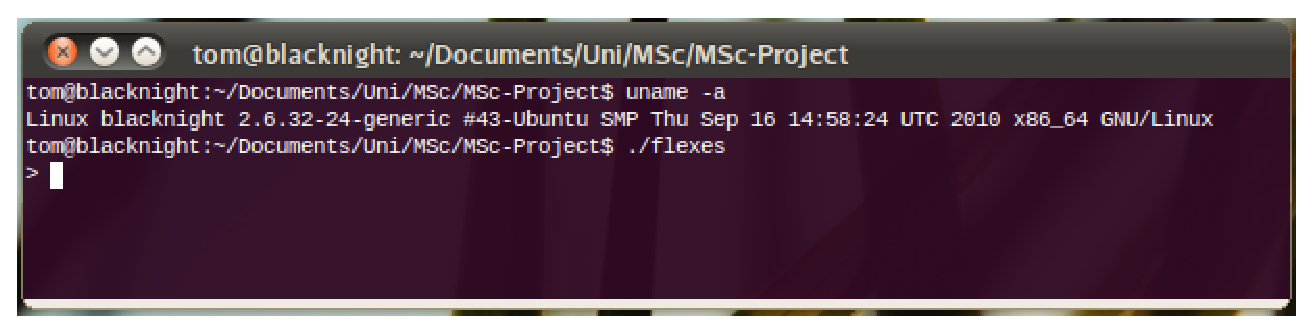
\includegraphics[scale=0.75]{linux}
	\caption{Running Ubuntu Linux, along with the compiler in text mode}\label{fig:linux}
\end{figure}
The compiler can also take an argument in the form of a flex file:
\begin{figure}[H]
	\centering
	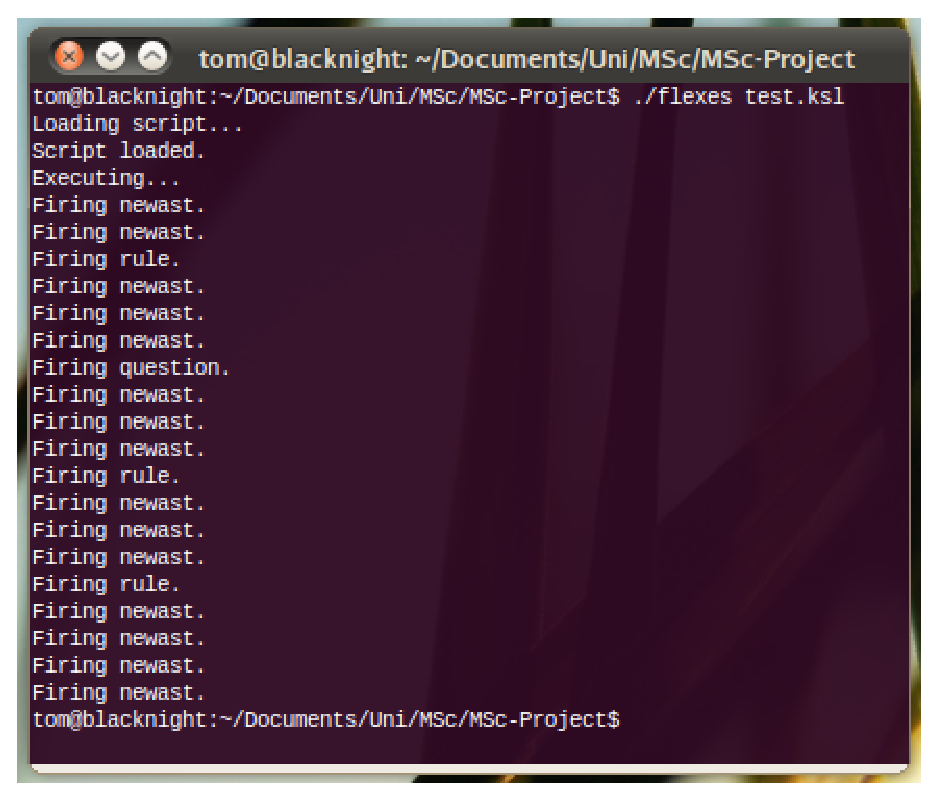
\includegraphics[scale=0.75]{flexes}
	\caption{The compiler (flexes) running a test script, without output.}\label{fig:flexes}
\end{figure}
In figure \ref{fig:flexes}, the compiler is reading from a source file that has been passed as an argument.\\
\\
Because the compiler is simple a source program without a graphical user interface, it doesn't make use of any library from Gnome or KDE.  If one wanted, a client could be built using GTK (Gnome) or QT (KDE) that would hook onto the flexes compiler.
\section{What could have been done better?}\label{sec:con:better}
In hindsight, the project could have gone further based on a greater amount of research at the start.  Whilst there is a lot of material on creating a compiler, many of them go deep into the theoretical side, rather than anything practical that can be put into use, and then learn from that.


\bibliographystyle{plainnat}
\bibliography{sample}
\end{document}



